\chapter{\textsc{Echantillonnage du signal d'erreur }}
\section{\textsc{La plage de valeurs de $T_e$}}

\par Pour déterminer cette plage de valeurs on doit calculer les valeurs propres du système de la boucle d'asservissement vu précédemment. Les pôles calculés par MATLAB valent :$ 
   \left \{
   \begin{array}{r c l}
      p_1  & = & -8.8730 \\
      p_2 & = & -1.1270
   \end{array}
   \right .$ 
   On prend le pôle dominant soit $p_2$  et :
   
   \begin{center}
   		$\frac{1}{|p_2|}<T_e<|p_2| \Rightarrow  0.28175 <T_e< 1.127 $
   \end{center}
  
\section{\textsc{Vérification de l'analyse avec MATLAB/SIMULINK}}

\subsection{Visualisation}

\begin{center}
	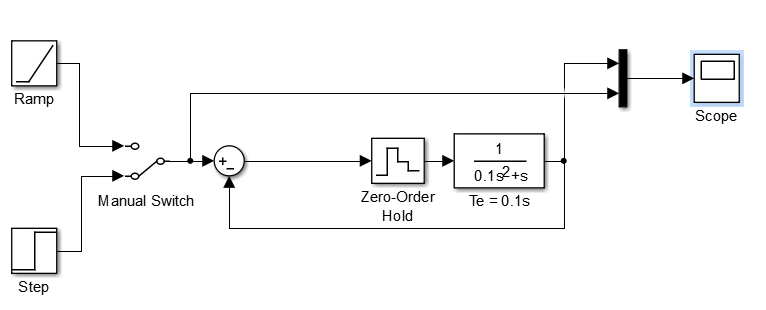
\includegraphics[scale=0.5]{shem11.png}
	\captionof{figure}{\textit{Schema simulink du système échantillonné pour différentes valeurs de $T_e$ \\}}
	\label{fig8} 
	\end{center}
	
	\begin{center}
	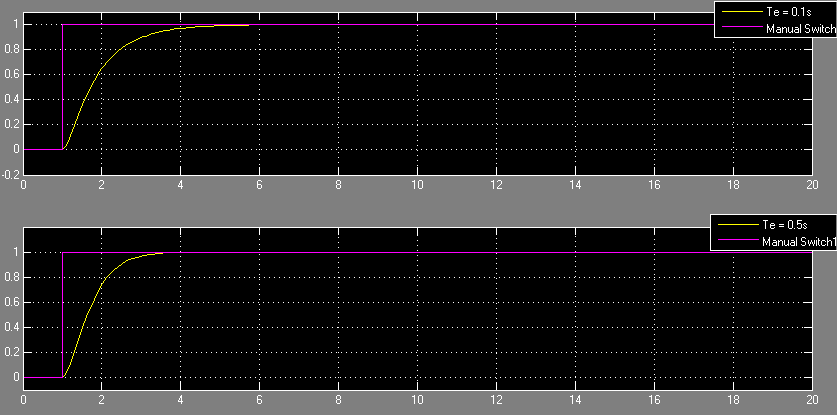
\includegraphics[scale=0.4]{simu11.png}
	\captionof{figure}{\textit{Réponses simulink de $s(t)$ pour de $T_e=0.1s$ et $T_e=0.5s$ \\}}
	\label{fig9} 
	\end{center}
	
	\begin{center}
	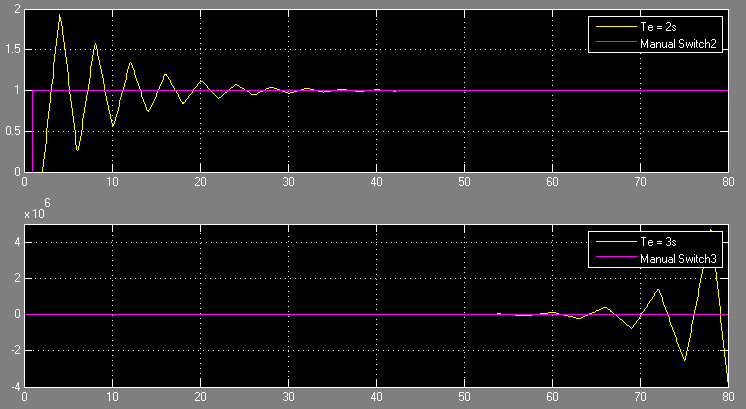
\includegraphics[scale=0.5]{simu22.png}
	\captionof{figure}{\textit{Réponses simulink de $s(t)$ pour de $T_e=2s$ et $T_e=3s$ \\}}
	\label{fig10} 
	\end{center}

\subsection{Commentaires}

\par Le système asservi diverge pour $T_e = 3 s$,  pour $T_e = 2 s$ il possède plusieurs oscillations et tarde à converger donc ces deux cas seront écartés.\\

   	
%	\begin{center}
%	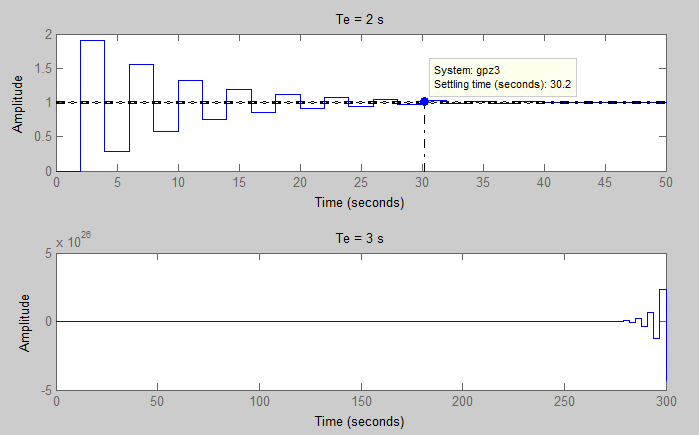
\includegraphics[scale=0.5]{mat2.png}
%	\captionof{figure}{\textit{Réponses $s(t)$ pour de $T_e=2s$ et $T_e=3s$ \\}}
%	\label{fig7} 
%	\end{center}

Il nous reste à comparer entre la réponse à $T_e=0.1s$ et à  $T_e=0.5s$, comparons leurs temps de réponses respectifs:\\
   
   	
%	\begin{center}
%	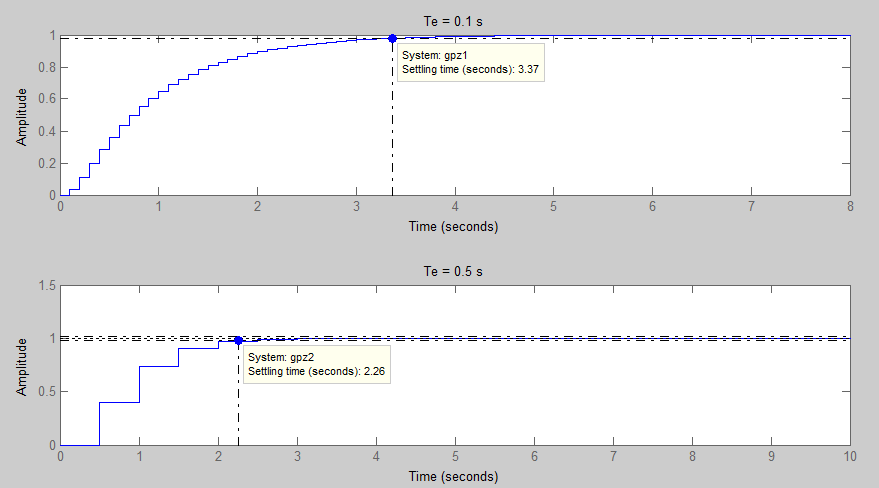
\includegraphics[scale=0.5]{mat1.png}
%	\captionof{figure}{\textit{Réponses $s(t)$ pour de $T_e=0.1s$ et $T_e=0.5s$ \\}}
%	\label{fig8} 
%	\end{center}
	
\par Il est clair qu'on écartera l'échantillonnge à $T_e=0.1$ et on retiendra celui à $T_e=0.5$ car le premier possède un temps de réponse $t_r=3.6113s$, il est plus grand que le temps de réponse que possède le système en temps continu contrairement à l'échantillonnage à $T_e=0.5 $ qui possède un temps de réponse $t_r = 2.8161 s$ et ne possède pas de dépassement,alors il respecte toutes les performances du système en temps continu.\\ 	
	

\textbf{Nota :} \label{section 2.2.2} \hyperref[Annexe A]{voir Annexe A} pour une analyse du système asservi discrétisé avec la commande MATLAB "c2d" et sur SIMULINK en utilisant le bloc LTI. On remarquera que le système asservi discrétisé garde les mêmes dynamiques que le système asservi echantillonné vu en dessus.

\section{\textsc{Visualisation de $s(t)$ pour la consigne $e_{ref}$}}

	\begin{center}
	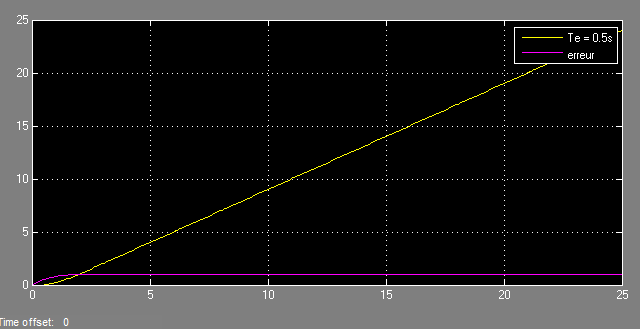
\includegraphics[scale=0.5]{simu3.png}
	\captionof{figure}{\textit{Réponse Simulink $s(t)$ à $T_e=0.5s$ en jaune pour la consigne $e_{ref}=e_1t$ et l'erreur $\epsilon (t) $ en mauve. \\}}
	\label{fig11} 
	\end{center}

\textbf{Conclusion:L'erreur de traînage vaut toujours $e_1$}

\section{\textsc{La démonstration}}
\par En se servant du tableau des transformées en Z on obtient :

\begin{center}
	
$\overline{B_0G}(z^{-1}) = \frac{( \tau - e^{\frac{-T_e}{\tau}}-\tau + T_e )z^{-1} ( 1 + \frac{\tau - ( \tau - T_e ) e^{\frac{-T_e}{\tau}}}{\tau - e^{\frac{-T_e}{\tau}}-\tau + T_e} ) z^{-1}} {(1-z^{-1}) (1- ( e^{\frac{-T_e}{\tau}} ) z^{-1})}$\\[0.25 cm]
	
	$ \Rightarrow \left \{
   \begin{array}{r c l}
      a_1  = \tau - e^{\frac{-T_e}{\tau}}-\tau + T_e \\\\
      a_2 =  \frac{\tau - ( \tau - T_e ) e^{\frac{-T_e}{\tau}}}{\tau - e^{\frac{-T_e}{\tau}}-\tau + T_e} \\\\
      b_1 = e^{\frac{-T_e}{\tau}}
   \end{array}
   \right . $
			
\end{center}


\par Ce qu'on va faire c'est de transformer $\overline{B_0G}(z^{-1})$ en $\overline{B_0G}(z)$ et ensuite l'identifier avec la fonction de transfert $G(p)$ discrétisée sous MATLAB avec la commande "c2d" et qu'on appelera $Gz(z)$, nous obtenons:

	\begin{center}
	 		
			$\overline{B_0G}(z)= \frac{a_1 z + a_1a_2}{z^2 -(b_1+1)z-b_1} $ \\[0.25cm]
			$Gz(z)= \frac{0.4007 z+ 0.09596}{z^2 + 1.007 z+ 0.006738} $\\[0.25cm]
			L'identification nous donne les valeurs numériques suivantes : $\Rightarrow 
	 \left \{
   \begin{array}{r c l}
      a_1 = 0.4007 \\
      a_2 =   0.3395\\
      b_1 = 0.00674
   \end{array}
   \right . $
	\end{center}
  
  \section{\textsc{Analyse de la stabilité par le lieu des racines}}
  
\par En utilisant cette méthode on pourra facilement en déduire le domaine de stabilité du système asservi. On utilisera pour ça la commande MATLAB "rltool":

	\begin{center}
	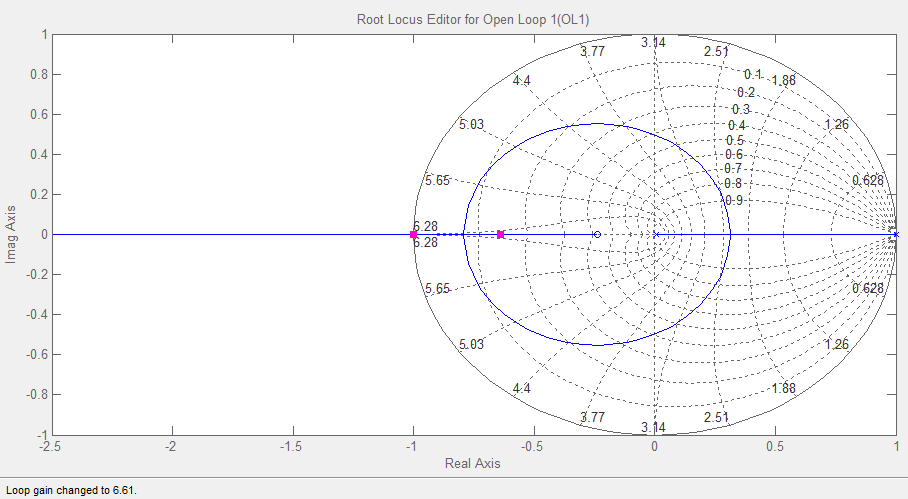
\includegraphics[scale=0.4]{rltool1.png}
	\captionof{figure}{\textit{ Le lieu des racines de la boucle fermée.\\}} 
	\label{fig12} 
	\end{center}

\par Puisque les deux pôles sont situé à l'intérieur du cercle unité alors le système asservi est asymptotiquement stable, de plus comme le montre la figure ci-dessus la stabilité est dissoute en appliquant un correcteur proprtionnel qui vaut plus de $ 6.61 $ cela explique que le domaine de stabilité du système bouclé est comprise entre :$K_p \in ]0,6.61]$.

%\section{\textsc{Calcul théorique de l'erreur de traînage $\epsilon_v$}}

